\subsubsection{Classification and regression tree}
	Classification and regression tree (\textbf{CART}) is an umbrella term used to refer to
	classification trees and regression trees.\cite{trees:umbrella}

	\bigskip\noindent The \textbf{CART} classifiers are a simple, yet powerful, classifier based around the tree structure. 
	They are often used within the datamining discipline in order to create a predictive model based for some preexisting data.
	The predictive model can then be used on new never seen before data in order to predict the most probable classification or value. 
	
	\bigskip\noindent Classification trees and regression trees are for all intent and purposes very similar, but some key differences are worth noteing. 
	One of these differences is in the outcome of their predictive model. 
	Classification trees, as the name may suggest, tries to pinpoint which \textit{class} an instance may belong to. 
	Whereas with regression trees the outcome of the model is a \textit{real number}, as the price of a certain item in a store. 
	
	\bigskip\noindent
	An example of decision tree applications can be seen as trying to predict the rating(1-10) of wine. 
	Given a dataset(Resource: \cite{mining:datasetexample} of preexisting knowledge, which include known attributes to a set of wines and their acoompanying rating.
	A decision tree may be constructred to generalize this knownledge in order to give a prediction of other wines. 	
		
	\begin{figure}[H]%
		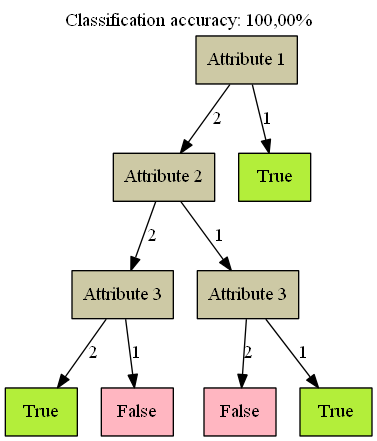
\includegraphics[width=\columnwidth]{images/TrivialDecisionTree.png}%
		\caption{Example classification tree from TDT4171. }%
		\label{fig:decisiontree}%
	\end{figure}
	
	\bigskip\noindent
	One example of a widely used CART algorithms comes from Ross Quinlan, the inventor of the ID3, C4.5 and C5.0 algorithms. \cite{quinlan:id3, quinlan:c45}
	All of whom use the notion of entropy in order to select the attribute to split for at a certain point in the tree. 
	They use entropy as a measurement of \textit{information gain} by selection a certain attribute at a given time during the algorithm. 
	The higher the gain is, the better do the attribute serve as an indicator of an instances' classification. 
	
